\documentclass[conference]{IEEEtran}
\IEEEoverridecommandlockouts
\usepackage{cite}
\usepackage{amsmath,amssymb,amsfonts}
\usepackage{algorithmic}
\usepackage{graphicx}
\graphicspath{{img/}}
\usepackage{textcomp}
\usepackage[table]{xcolor}
\usepackage{verbatim}
\usepackage{tabularx}
\usepackage{listings}
\usepackage{xcolor}
\usepackage{hyperref}
\hypersetup{
    colorlinks=true,
    linkcolor=blue,
    filecolor=magenta,      
    urlcolor=cyan,
}
 
\definecolor{codegreen}{rgb}{0,0.6,0}
\definecolor{codegray}{rgb}{0.5,0.5,0.5}
\definecolor{codepurple}{rgb}{0.58,0,0.82}
\definecolor{backcolour}{rgb}{0.95,0.95,0.92}
 
\lstdefinestyle{mystyle}{
    backgroundcolor=\color{backcolour},   
    commentstyle=\color{codegreen},
    keywordstyle=\color{magenta},
    numberstyle=\tiny\color{codegray},
    stringstyle=\color{codepurple},
    basicstyle=\ttfamily\footnotesize,
    breakatwhitespace=false,         
    breaklines=true,                 
    captionpos=b,                    
    keepspaces=true,                 
    numbers=left,                    
    numbersep=5pt,                  
    showspaces=false,                
    showstringspaces=false,
    showtabs=false,                  
    tabsize=2
}
\lstset{style=mystyle}

\def\BibTeX{{\rm B\kern-.05em{\sc i\kern-.025em b}\kern-.08em
    T\kern-.1667em\lower.7ex\hbox{E}\kern-.125emX}}
\begin{document}

\title{
 Cosmic\\Final Simulation and Real-time Code}
\author{\IEEEauthorblockN{Clay Buxton}
\IEEEauthorblockA{\textit{Computer Engineering, Computer Science} \\
\textit{Elizabethtown College}\\
Elizabethtown, PA \\
buxtonc@etown.edu}
\and
\IEEEauthorblockN{Kevin Carman}
\IEEEauthorblockA{\textit{Computer Engineering, Computer Science} \\
\textit{Elizabethtown College}\\
Elizabethtown, PA \\
carmank@etown.edu}
}
\maketitle

\section{Aspirations}
We introduced Cosmic as a fully simulated 8-bit microcomputer architecture that was designed to act like a physical chip, but be completely software based. We aspired to write everything from an instruction set, to an operating system for it, alongside a rich GUI environment and an assembler. Some of the early design constraints included a RISC-like instruction set containing less than 50 total instructions, the design to be derived from the Zilog Z80 and MOS 6502 microprocessors, a budget of \$0, and that timing would not be a constraint.

As development went on, our focus shifted to designing Cosmic to be a tool to learn both assembly and low level computing. The instruction set and architecture were mostly flushed out by this point, so we turned to improving the GUI environment, writing the assembler, and even writing some introductory labs that could be used to teach how Cosmic works.

In the end, all of our original design constraints were met except for the \$0 budget. We purchased a Raspberry Pi that was powerful enough to run Cosmic so that we could create and test a way for Cosmic to interface with the real-world through the GPIO pins on the Pi. Everything, including our architecture, GUI environment, and assembler, is currently in a working state.

\section{Real-time Code}
Three introductory labs were created to teach how to write assembly and utilize Cosmic in an educational environment. The labs are generated from a compact and clean LaTeX template, and are easily editable and reusable. They include information such as the lab objective, a prelab section that asks the students to familiarize themselves with specific instructions or other key aspect of Cosmic beforehand, a during lab section that lays out the problem the students must solve, a grading section that breaks down exactly what is required of the student for the lab, and a helpful links section that directs to Cosmic documentation and other helpful places.

All of the labs, their accompanying solutions, and the rest of the Cosmic source code can be found in our \href{https://github.com/clbx/Cosmic}{GitHub repository}.\\

\subsection{Basic Operations}
The first lab asks the student to calculate and the nth Fibonacci number. Since our processor, is only 8 bits, the following constraint is applied: 1 $\leq$ n $\leq$ 13. This lab teaches the basics of Cosmic, such as using instructions, variables, and loops in the assembler to carry out simple tasks. A sample solution is shown in Listing \ref{label1}.

\begin{lstlisting}[caption={Cosmic assembly to find the nth Fibonacci number.}, label = {label1}]
byte fib = 6
;The Fibonacci number we wish to calculate
byte counter = 2
byte first = 0
byte second = 1
;Initialize the first two numbers in the sequence to be 1
byte final = 0
JMP #08
end:
    MOV R0 final
    HCF
    ;End of program
MOV #1 R0
CMP fib
JZS #end
;Check to see if fib is 1
calculate:
    MOV first R0
    ADD second
    MOV second first
    MOV R0 second
    MOV fib R0
    CMP counter
    MOV second R0
    ;Needed since we store R0 in final
    JZS #end
    INC counter
    JMP #11
\end{lstlisting}

Since we are calculating the nth Fibonacci number, we stored our n, in this case 6, as fib. A Fibonacci number is calculated by adding together the previous two numbers in the sequence, so we stored the first and second numbers of the sequence accordingly. We defined a counter variable to keep track of which Fibonacci number we are on, and we initialize it to two because if we want the first number in the sequence, we can just return 1 without any calculations. Lastly, we defined a final variable to store our answer in. We then defined an end loop, which is only called after we have generated our answer, to store our final answer in. The MOV, CMP, and JZS instructions following the end of the end loop act as an if statement to check is fib is equal to 1. If it is not, then we head into the calculate loop. This loop moves our first variable into the accumulator and adds the second to it. Then it moves the second variable to the first, and the accumulator to the second. It then checks to see if we have calculated the nth Fibonacci number or not. If we need to continue calculating, the counter is incremented and JMP is called to bring us back to the start of the calculate loop. If the answer has been found, the end loop is called and the program ends after it executes. After the program ends, 8, the 6th Fibonacci number, should be stored in the final variable.

After a program like the one found in Listing \ref{label1} is written, it is as simple as clicking Assemble in the Cosmic editor to assemble the code into machine code and load it into the memory editor. All the user has to do afterwards is simply click Run to start executing the program.

\subsection{Basic Graphics}
The second lab asks the student to write a program to output a gradient to the Cosmic video screen. Since Cosmic's video output works by reading the video memory for brightness values for each pixel from 0x00 to 0xFF, the student much loop through the video memory and store either decreasing or increasing values of brightness for the pixels. This lab again reinforces the basics of Cosmic and introduces the usage of the video output. A sample solution is shown in Listing \ref{label2}.

\begin{lstlisting}[caption={Cosmic assembly to output a gradient to the video screen.}, label = {label2}]
byte brightness = FE
;Start at full brightness -1 so that the program terminates accordingly.
word start = 8000
;Starting pixel
MOVX #BFFF R0
;Store the end location of the video memory.
loop:
	MOV brightness @start
	;Set the brightness of this pixel
	DEC brightness
    DEC brightness
    ;Decrement the brightness by two because the video out is 64x64
	INCX start
	CMPX start
	JNZ #loop
	;Repeat until the brightness reaches 0
HCF
;End of program
\end{lstlisting}

Since Cosmic's video screen is 64x64, we define our initial brightness to be 0xFE. We also define a word, 16 bits instead of 8 bits, starting location for the beginning of the video memory. We then MOV the end location of the video memory to the 16-bit accumulator as a reference. Next, we defined a loop to MOV the current brightness value to the current pixel in video memory. We then decrement the brightness variable twice, since each line of the video screen is only 64 pixels long, and increment our position in video memory. Lastly, we compare our position in video memory to the accumulator, since we stored the end location there, to determine if we should continue drawing or end the program. The outcome is a smooth gradient as can be seen in Figure \ref{fig:gradient}.

\begin{figure}[h!]
	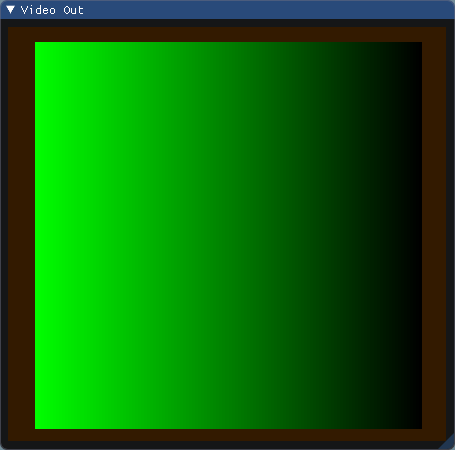
\includegraphics[width=\linewidth]{lab_2_solution}
	\caption{The gradient produced in Lab 2.}
	\label{fig:gradient}
\end{figure}

\subsection{Real-world Interfacing}
The third and final lab asks the student to write a simple program to read input from a button hooked up to a Raspberry Pi and turn on an LED when input is detected. This lab introduces the student to interfacing Cosmic with something physical like a Raspberry Pi. Even though the task in the lab is simple, it opens up a whole new world of opportunities to explore. In Cosmic, Raspberry Pi GPIO pins are mapped to the values in memory from 0xC402 to 0xC41E. The most significant bit in the GPIO bytes signify whether the pin is an input or an output. The remaining 7 bits set it ON or OFF. If the 7 bits equal zero, then the pin if OFF. If they equal something greater than 0, then it is ON. A sample solution is shown in Listing \ref{label3}.

\begin{lstlisting}[caption={Cosmic assembly to interface with a Raspberry Pi.}, label = {label3}]
word inputLoc = C402
word outputLoc = C403
start:
	MOV inputLoc R0
    AND FF
	JNZ #turnON
    JMP #turnOFF
turnON:
	MOV FF outputLoc
    JMP #start
turnOFF:
	MOV 80 outputLoc
	JMP #start
\end{lstlisting}

Since the pins are mapped directly to memory in Cosmic, we defined two words to store the input and output locations of the pins we want to use. We then defined a start loop that determines if the LED should be turned on or off based on ANDing the input value with 0xFF and jumping accordingly. If the LED needs to be turned on, the loop jumps to the turnON label that MOVs 0xFF to the output location and jumps back to the start loop. If the LED needs to be turned off, the loops jumps to the turnOFF label that MOVs 0x80 to the output location and jumps back to the start loop. This allows the student to infinitely poll the input from the Raspberry Pi.

\section{Outcome}
In the end, we could not be happier with the product we delivered. We committed a significant amount of time to Cosmic throughout the last year to get it to where it is now and learned a lot along the way. We hope that Cosmic, or even just the idea of Cosmic, enables and encourages more people to get involved with the retro-computing community and to learn about low level computer design and functionality.

\end{document}